% Few-shot error vs k on the synthetic population (spread 1): numbers from
% ../results/loro_spread1.txt (popsim.py loro), medians over 8 held-out robots x 3 subsets.
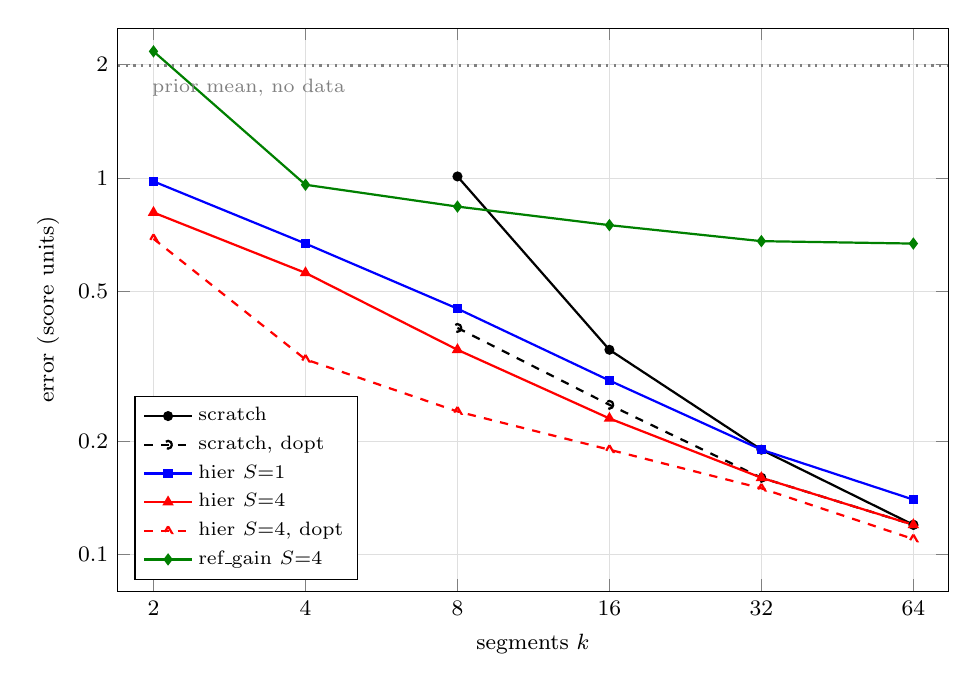
\begin{tikzpicture}
\begin{loglogaxis}[
  width=\columnwidth, height=0.72\columnwidth,
  xlabel={segments $k$}, ylabel={error (score units)},
  xtick={2,4,8,16,32,64}, xticklabels={2,4,8,16,32,64},
  ytick={0.1,0.2,0.5,1,2}, yticklabels={0.1,0.2,0.5,1,2},
  ymin=0.08, ymax=2.5, xmin=1.7, xmax=75,
  legend style={font=\scriptsize, at={(0.02,0.02)}, anchor=south west, cells={anchor=west}},
  grid=major, grid style={gray!25}, tick label style={font=\footnotesize}, label style={font=\footnotesize},
]
\addplot[black, thick, mark=*, mark size=1.4] coordinates {(8,1.01) (16,0.35) (32,0.19) (64,0.12)};
\addlegendentry{scratch}
\addplot[black, thick, dashed, mark=o, mark size=1.4] coordinates {(8,0.40) (16,0.25) (32,0.16) (64,0.12)};
\addlegendentry{scratch, dopt}
\addplot[blue, thick, mark=square*, mark size=1.3] coordinates {(2,0.98) (4,0.67) (8,0.45) (16,0.29) (32,0.19) (64,0.14)};
\addlegendentry{hier $S{=}1$}
\addplot[red, thick, mark=triangle*, mark size=1.6] coordinates {(2,0.81) (4,0.56) (8,0.35) (16,0.23) (32,0.16) (64,0.12)};
\addlegendentry{hier $S{=}4$}
\addplot[red, thick, dashed, mark=triangle, mark size=1.6] coordinates {(2,0.69) (4,0.33) (8,0.24) (16,0.19) (32,0.15) (64,0.11)};
\addlegendentry{hier $S{=}4$, dopt}
\addplot[green!50!black, thick, mark=diamond*, mark size=1.6] coordinates {(2,2.17) (4,0.96) (8,0.84) (16,0.75) (32,0.68) (64,0.67)};
\addlegendentry{ref\_gain $S{=}4$}
\addplot[gray, dotted, thick, domain=1.7:75] {0.05};
\addplot[gray, dotted, thick, domain=1.7:75] {1.99};
\node[gray, font=\scriptsize, anchor=south west] at (axis cs:1.9,0.052) {full grid};
\node[gray, font=\scriptsize, anchor=north west] at (axis cs:1.9,1.95) {prior mean, no data};
\end{loglogaxis}
\end{tikzpicture}
